%%%%%%%%%%%%%%%%%%%%%%%%%%%%%%%%%%%%%%%%%%%%%%%%%%%%%%%%%%%%%%%%%%%%
%% I, the copyright holder of this work, release this work into the
%% public domain. This applies worldwide. In some countries this may
%% not be legally possible; if so: I grant anyone the right to use
%% this work for any purpose, without any conditions, unless such
%% conditions are required by law.
%%%%%%%%%%%%%%%%%%%%%%%%%%%%%%%%%%%%%%%%%%%%%%%%%%%%%%%%%%%%%%%%%%%%

\documentclass{beamer}
\usetheme[]{default}
\usepackage{marvosym}
\usepackage[utf8]{inputenc}
\usepackage[
  main=english, %% By using `czech` or `slovak` as the main locale
                %% instead of `english`, you can typeset the
                %% presentation in either Czech or Slovak,
                %% respectively.
]{babel}        %% typeset as follows:
%%
%%   \begin{otherlanguage}{czech}   ... \end{otherlanguage}
%%   \begin{otherlanguage}{slovak}  ... \end{otherlanguage}
%%
%% These macros specify information about the presentation
\title{Report Attività Formative e di Ricerca} %% that will be typeset on the
\subtitle{II Anno Dottorato in Matematica e Informatica} %% title page.
\author{Davide Spataro}
%% These additional packages are used within the document:
\usepackage{ragged2e}  % `\justifying` text
\usepackage{booktabs}  % Tables
\usepackage{tabularx}
\usepackage{tikz}
\newcommand*\circled[1]{\tikz[baseline=(char.base)]{
            \node[shape=circle,draw,inner sep=0.3pt] (char) {#1};}}
\usetikzlibrary{positioning,chains,fit,shapes,calc}
\usetikzlibrary{calc, shapes, backgrounds}
\usepackage{amsmath, amssymb}
\usepackage{url}       % `\url`s
\usepackage{listings}  % Code listings
\frenchspacing
\begin{document}
  \frame{\maketitle}

 \AtBeginSection[]{
  \begin{frame}
  \vfill
  \centering
  \begin{beamercolorbox}[sep=8pt,center,shadow=true,rounded=true]{title}
    \usebeamerfont{title}\insertsectionhead\par%
  \end{beamercolorbox}
  \vfill
  \end{frame}
}

    \section{Visualization For Extremely Large-Scale
Scientific Computing}
    \subsection{Platform Description}
   
  %----BEGIN FRAME-----
  \begin{frame}{Introduction}
\textbf{\textit{ VeLASSCo}} is  a 3.1M EU funded\footnote{\textit{(FP7/2007-2013)}} project

\begin{block}{Consortium}
	The consortium is lead and coordinated by \textbf{CIMNE} (\textit{Spain}) and partecipated by: 
	\begin{itemize}
		\item \textbf{Univerisity of Edinburgh} (\textit{UK}) - School of Engineering
		\item \textbf{SINTEF} - Dept. of Applied Mathematics (\textit{Norway})
		\item \textbf{Inria} (\textit{France})
		\item \textbf{Fraunhofer} (\textit{Germany})- Dept. Interactive Engineering Technologies (IET)
		\item \textbf{Jotne} (\textit{Norway})
		\item \textbf{Atos} (\textit{Spain})
	\end{itemize}
\end{block}


\end{frame} %----END FRAME-----   
   
  %----BEGIN FRAME-----
  \begin{frame}{Introduction}
		\begin{exampleblock}{\textbf{\textit{ VeLASSCo}} objective is to perform}	
	 		\textbf{pre-processing} and \textbf{visualization} of \textbf{very large} simulations.
		\end{exampleblock}	
		
		 \begin{figure}
			 \centering
			   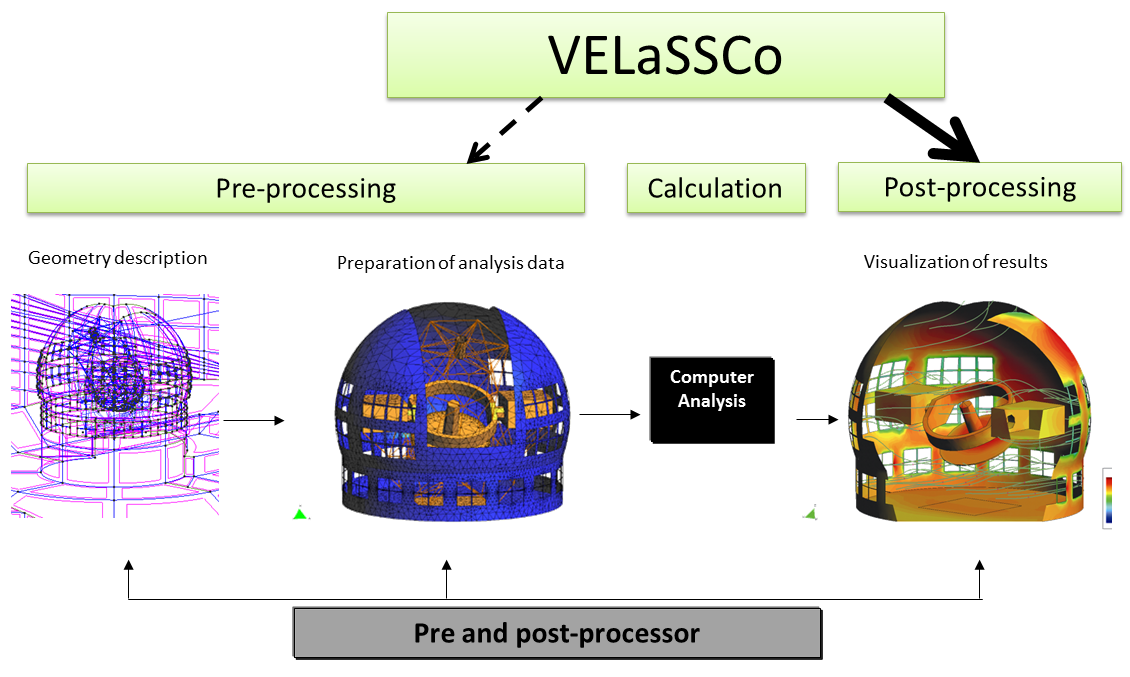
\includegraphics[width=\textwidth]{velassco-context}
		 \end{figure}

\end{frame} %----END FRAME-----

  %----BEGIN FRAME-----
  \begin{frame}{How?}
		\begin{exampleblock}{\textbf{\textit{ VeLASSCo}} brings together	\textbf{Big-Data} and \textbf{Simulation}}
		

		\begin{itemize}
			\item ``Big-Data" (phylosophy more than technology) addresses post-processing in a distributed way making the system \textbf{highly scalable}
			\item all post-processing algorithm are parallel (map-reduce scheme)
			\item Parallel Rendering and GPGPU to achieve high throughput rendering rate and interactive visualization
		\end{itemize}

		\end{exampleblock}	
		
		

\end{frame} %----END FRAME-----

 %----BEGIN FRAME-----
  \begin{frame}{Achitercture}
		\begin{exampleblock}{\textbf{\textit{ VeLASSCo}} Architecture}
	\begin{itemize}
	\item Data-Layer - HDFS/HBASE + Flume (Simulation Data Ingestion)
	\item Data Analytics - Map-Reduce Yarn/Hadoop + post-processing parallel algorithms 
	\item Visualization - \textbf{My work!} 
	\end{itemize}
		 \begin{figure}
			 \centering
			   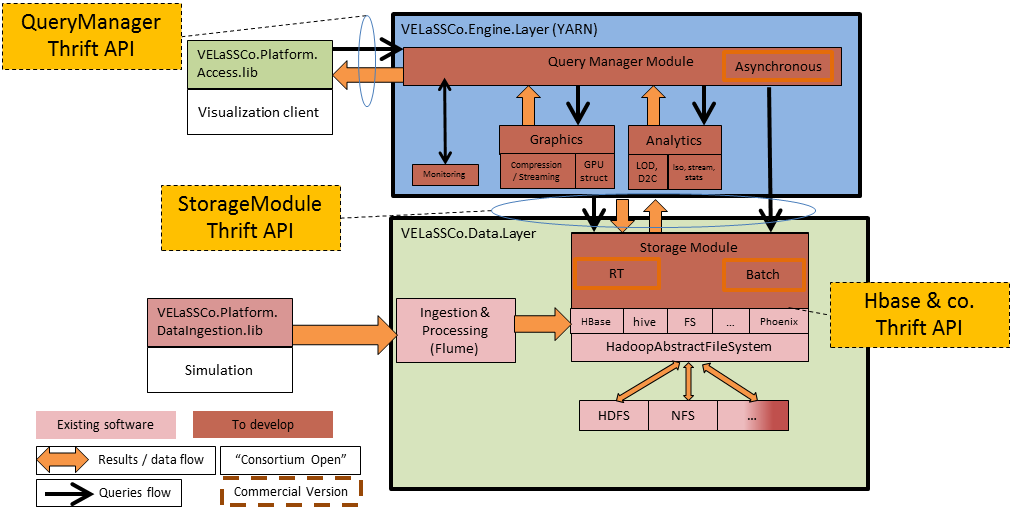
\includegraphics[scale=0.3]{velassco-platform-os}
		 \end{figure}

		\end{exampleblock}	
		
		

\end{frame} %----END FRAME-----

\subsection{Visualization}
 %----BEGIN FRAME-----
  \begin{frame}{Visualization}
		\begin{exampleblock}{Classic Workflow does not work}
	\begin{itemize}
		\item Visualization performed at client side
		\item Data are moved from HPC to the client workstation
	
		\item \textit{Dealing with such huge dataset makes this approach infeasible}
		\item \textit{No single GPU or shared memory machine can handle such amount of data (billions of graphics primitives)}
	\end{itemize}


		\end{exampleblock}	
		\begin{alertblock}{Proposed Solution: \textit{\textbf{Parallel Rendering}}}
	\begin{itemize}
		\item Rendering is performed offline inside the platform
		\item Dataset rendering responsibility is \textbf{shared among} a number of \textbf{dedicated visualization node}
		\item No need to move huge amount of data outside the platform
	\end{itemize}


	\end{alertblock}	
		

\end{frame} %----END FRAME-----


 %----BEGIN FRAME-----
  \begin{frame}{Visualization}
		\begin{exampleblock}{Parallel Rendering: $3$ Types}
		\begin{itemize}
			\item Sort-First: the screen is divided into tiles. Each tile is assigned a full pipeline  (SLI)
			\item Sort-Middle: Primitive are divided \textbf{arbitrarly} among all nodes and  trasformed triangles are eventually gathered by a \textbf{single} rasterizer (Mobile GPUs).
			\item Sort-Last: Arbitrary division, but each node produces a single framebuffer  (complet the rendering of a data subset). Framebuffers are then composed in order to form the final image. \textbf{Composition can be performed in parallel!} 
		\end{itemize}

		\end{exampleblock}	
	
		

\end{frame} %----END FRAME-----

 %----BEGIN FRAME-----
  \begin{frame}{Visualization: Solution}
		
\begin{columns}[T] % align columns
\begin{column}{.48\textwidth}

\begin{itemize}
			\item The to be rendered dataset can be divided in order to ensure \textbf{load balancing} (the whole dataset may be in a single screen tile)


		\end{itemize}
\begin{exampleblock}{Adopted solution is Sort-Last}
		\begin{itemize}
			
			\item Each rendering node produces a framebuffer using an independent pipeline and possibly heterogeneous HW
			\item Composition of the final image is performed in parallel (reduction)

		\end{itemize}
		
		

		\end{exampleblock}	
\end{column}%
\hfill%
\begin{column}{.58\textwidth}

\begin{figure}
			 \centering
			   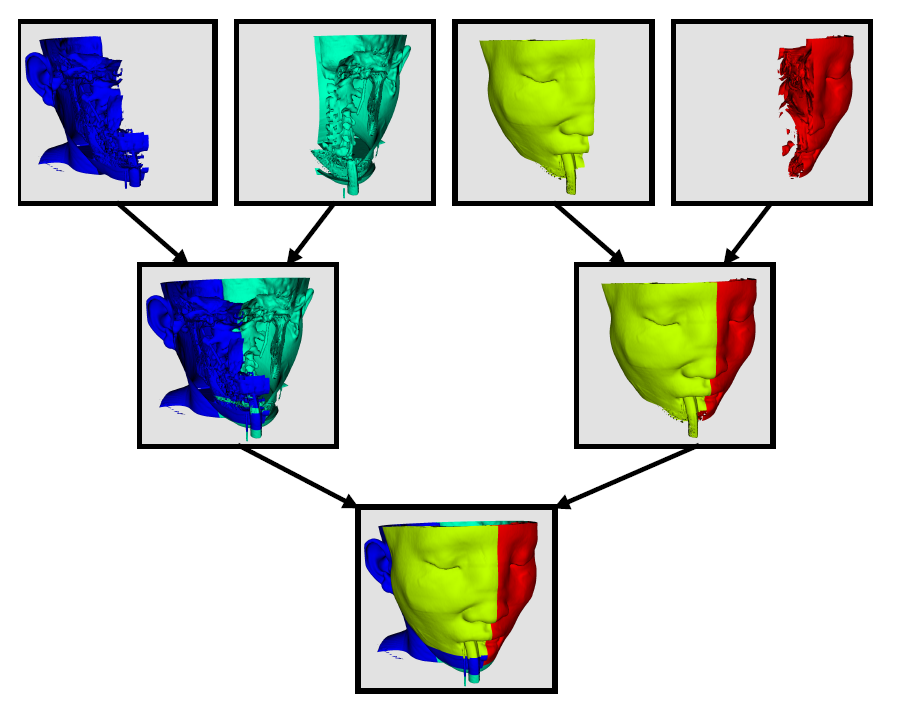
\includegraphics[scale=0.2]{parrend}
		 \end{figure}

\end{column}%
\end{columns}		
		
		
	
		
\end{frame} %----END FRAME-----


 %----BEGIN FRAME-----
  \begin{frame}{Visualization: Challenges}
		\begin{exampleblock}{Parallel Rendering on top of HBASE}
	\begin{itemize}
		\item Parallel Rendering requires direct control and mainipulation of RAW data
		\item Big-Data map-reduce \textbf{hides} parallelism and distribution of data
	\end{itemize}
	\end{exampleblock}
			
	\begin{alertblock}{HBase Coprocessor}
		Visualization runs in Coprocessor container which allows custom code to run for each region-server(i.e. node). 



	\end{alertblock}	
		

\end{frame} %----END FRAME-----

%----BEGIN FRAME-----
  \begin{frame}{Visualization: Results}
		\begin{exampleblock}{A prototype was developed}
	\begin{itemize}
		\item Test case is a Fluidized Bed simulation (Largest available \textbf{500GB})
		\item Parallel Rendering using 16 nodes (software rendering \Frowny{} ) 
		\item Preliminary Results show good rendering performance ($triangles \times s^{-1}$) 
	\end{itemize}
	\end{exampleblock}
			
	\begin{alertblock}{Next Deliverable}
	\begin{itemize}
		\item Develop a load balancing module which automatically split the work among the rendering nodes s.t. work and communication is minimized (store precomputed metadata).
		\item HW rendering + GPGPU preprocessing
		
	\end{itemize}



	\end{alertblock}	
		

\end{frame} %----END FRAME-----

\section{Tracking particle-like Objects}



%----BEGIN FRAME-----
  \begin{frame}{Introduction}
		\begin{exampleblock}{Why tracking such Objects?}
		Particle tracking is an important subtask in numerous investigation regarding sub-micron particles, microspheres and molecules under microscopic observation.
		From trajectories important \textbf{dynamic} and \textbf{kinematic} motion properties can be computed.
			
		\end{exampleblock}		

		\begin{alertblock}{Research Activity}
			
		\begin{itemize}
			 \item Joint research with a group from the \textit{Institute of Bioengineering, University of Edinburgh}
			 \item Work Submitted at the \textit{Parallel and Distributed Computing Conference PDP2017}
			 \item Case study on the investigation of the \textit{B. subtilis} chemiotaxis

			\end{itemize}
			
		\end{alertblock}	
		
\end{frame} %----END FRAME-----


%----BEGIN FRAME-----
  \begin{frame}{Algorithm Descritpion}
		\begin{exampleblock}{The Proposed Algorithm}
			 produces a set of trajectories from time-lapse video \textit{frames}. 
			\begin{itemize}
				\item Traceable Object are described by a centroid and a \textit{bounding box}
				\item \textit{bounding box} describes geometrical properties of the object (shape area/volume etc.)
				\item The algorithm is based on centroid/shape minimization difference method
			\end{itemize}
			
		\end{exampleblock}		

		
		
\end{frame} %----END FRAME-----

%----BEGIN FRAME-----
  \begin{frame}{Algorithm Descritpion}
		\begin{exampleblock}{Algorithm Formalization}
Let $P=P_1 \cup P_2 \cup \ldots \cup P_n$ be the set of frames, $\mathcal{D} :  P \times P \mapsto \mathbb{R}$ the \textit{distance} function. $P_i = \{p^j_i \; | \; 1 \leq j\; \}$ indicates all particles at time $i$. $\mathcal{D}(p,q)$ measures the likeliness that a particle $p$ has been transformed into $q$ as a result of the application of a number of geometrical transformations. 
Iterativelly processes at each step two set $M_i$ and $P_i$.$M_i$ is the set of ``under construction" trajectories. Informally, it tries to augment an element of $M_i$ using a particle at frame $i$ s.t. the distance function is minimized.

		\end{exampleblock}		

		
		
\end{frame} %----END FRAME-----

%----BEGIN FRAME-----
  \begin{frame}{Algorithm Descritpion}
		\begin{exampleblock}{The Algorithm as  Graph Problem}
			The problem at hand can be viewed as a variant of the famous \textit{assignment problem} and more specifically it consists in finding a minimum weight matching in  a weighted bipartite directed graph $G=(V,E)$ where $V={M_i} \cup P_i$ is the set of nodes and ${M_i}, P_i$ are the two partitions, $E = {M_i} \times P_i$ s.t. $e \in E, \mathcal{D}(e) \in \mathbb{R}$.
A valid matching $S \subseteq E$ must satisfy the following: 
\begin{equation}
\forall (u,v) \in S 
\left\{
  \begin{array}{lr}
   (w,x) \in S,\; v=x\Longleftrightarrow u=w\\
   \mathcal{D}(u,v) = \min_{x \in V_2} \mathcal{D}(u,x)  \\
    \nexists \: (w,v) \in E \: \mbox{s.t.} \: \mathcal{D}(w,v) < \mathcal{D}(u,v)
  \end{array}
\right.
\label{matchConstraints}
\end{equation}

		\end{exampleblock}		

		
		
\end{frame} %----END FRAME-----

%----BEGIN FRAME-----
  \begin{frame}{Algorithm Descritpion}
		
			If we denote the matching procedure as the following recurrence relation $  M_i \lozenge P_{i+1} = (T_{i+1},M_{i+1}) $, $M_0=P_0$, then the  tracking algorithm can be summarized as $(T_n,M_n) = M_{n-1} \lozenge P_{n}=(((P_0 \lozenge P_1)\lozenge P_2) \lozenge \ldots \lozenge P_n)$.

\begin{alertblock}{Under the assumption of associativity}
the algorithm can be parallelized as it is, using the parallel reduction design scheme.

\end{alertblock}


		
\end{frame} %----END FRAME-----

  \begin{frame}{Algorithm Descritpion - Matching}

\begin{figure}
\centering
	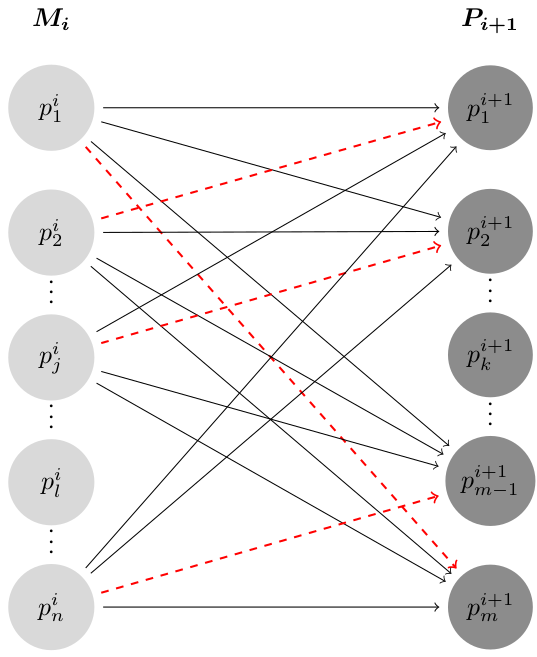
\includegraphics[scale=0.23]{matching}
	\caption{Dashed red arrows highlight the solution $S$. For instance, the trajectory $t_*=p^s_a \leadsto p^i_1$  is lengthened by $p^{i+1}_m$ becoming $t=p^s_a \leadsto p^i_1 \to p^{i+1}_m$.
Note that, for the sake clarity, and weights and arrows for the unmatched   nodes are omitted.}
	\end{figure}	
	
\end{frame} %----END FRAME-----



%----BEGIN FRAME-----
  \begin{frame}{ Extended Cellular Automata (XCA) - Image Processing Framework}
		Since images are a common source of data an image processing framework based on XCA was developed.
		\begin{itemize}
			\item Works for $n$-dimensional \textit{images}
			\item Allows seamless convolution and filters application on images 
			\item Filters and convolutional kernels can be user-specified
			\item Is it automatically executed in parallel (GPGPU and shared memory)
		\end{itemize}
\begin{columns}[T] % align columns
\begin{column}{.48\textwidth}

\begin{figure}
			 \centering
			   
\includegraphics[scale=0.45]{bacteriasmall}
		 \end{figure}
\end{column}%
\hfill%
\begin{column}{.58\textwidth}

\begin{figure}
			 \centering
			   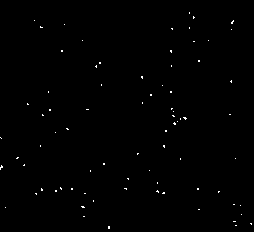
\includegraphics[scale=0.45]{bacteriasmall_threshold}
		 \end{figure}

\end{column}%
\end{columns}	

		
\end{frame} %----END FRAME-----



%----BEGIN FRAME-----
  \begin{frame}{ Motility Analysis of \textit{B. subtilis}}
		In order to validate the proposed algorithm and framework on the analysis of \textit{B. subtilis} in a microfluidic device. Time-lapse video is composed of 4100 frames.
		
		\begin{itemize}
			\item Images were preprocessed and bacteria segmented by means a composition of \textit{threshold}, \textit{contrast stretch}, and a number of convolutional filters.
			\item The proposed algorithm was applied in order to reconstruct the trajectories 
			\item Distance function used was a linear combination of centroid displacement and shape difference
		\end{itemize}

		
\end{frame} %----END FRAME-----

%----BEGIN FRAME-----
  \begin{frame}{ Motility Analysis of \textit{B. subtilis} - Results}
Trajectories were analysed using two different and standard methods. Three motility parameters were taken in consideration:
\begin{enumerate}
\item Mean Swimming Time
\item Mean Run Time
\item Tumble Time
\end{enumerate}
The values obtained from the tracked trajectories are in accordance with those available in the literature, confirming that the trajectories were tracked with good accuracy.
ds

		
\end{frame} %----END FRAME-----


%----BEGIN FRAME-----
  \begin{frame}{  Collective view of the tracked trajectories}


\begin{figure}
			 \centering
			   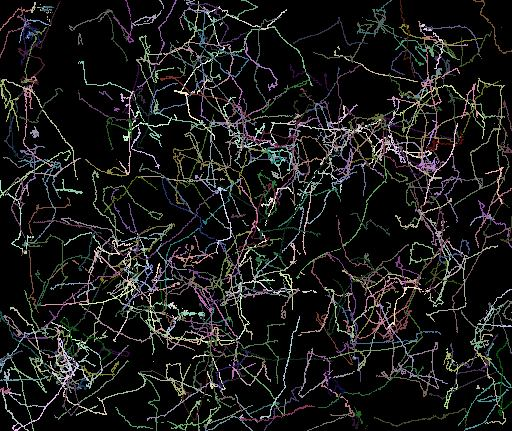
\includegraphics[scale=0.45]{../result}
		 \end{figure}

		
\end{frame} %----END FRAME-----

\begin{frame}{}
  \centering \Huge
  \emph{Thanks for your attention!}
\end{frame}



%      \begin{tikzpicture}[overlay,remember picture]
%        \node[anchor=south east,xshift=-30pt,yshift=35pt]
%          at (current page.south east) {
%            \includegraphics[width=35mm]{resources/jabberwocky-light}
%          };
%      \end{tikzpicture}


\end{document}
